\documentclass{article}
\usepackage{arxiv}

\usepackage[utf8]{inputenc}
\usepackage[english, russian]{babel}
\usepackage[T1]{fontenc}
\usepackage{url}
\usepackage{booktabs}
\usepackage{amsfonts}
\usepackage{nicefrac}
\usepackage{microtype}
\usepackage{lipsum}
\usepackage{graphicx}
\usepackage{natbib}
\usepackage{doi}



\title{Использование пространственно-временных зависимостей для мониторинга аддитивного производства с применением глубокого обучения}

\author{Vladislav Soldatov\\
	\texttt{worklikewalkietalkie@gmail.com} \\
	%% examples of more authors
	\And
	  Dmitry Kropotov \\
	\texttt{dmitry.kropotov@gmail.com} \\
	%% \AND
	%% Coauthor \\
	%% Affiliation \\
	%% Address \\
	%% \texttt{email} \\
	%% \And
	%% Coauthor \\
	%% Affiliation \\
	%% Address \\
	%% \texttt{email} \\
	%% \And
	%% Coauthor \\
	%% Affiliation \\
	%% Address \\
	%% \texttt{email} \\
}
\date{}

\renewcommand{\shorttitle}{\textit{arXiv} Template}

%%% Add PDF metadata to help others organize their library
%%% Once the PDF is generated, you can check the metadata with
%%% $ pdfinfo template.pdf
\hypersetup{
pdftitle={Использование пространственно-временных зависимостей для мониторинга аддитивного производства с применением глубокого обучения},
pdfsubject={q-bio.NC, q-bio.QM},
pdfauthor={Vladislav Soldatov, Dmitry Kropotov},
pdfkeywords={Additive manufacturing, Laser Powder Bed Fusion, Online
monitoring, Flaw detection, Porosity prediction, Spatial-temporal Modeling},
}

\begin{document}
\maketitle

\begin{abstract}
	Мониторинг процессов аддитивного производства в режиме реального времени необходим для обеспечения качества деталей и предотвращения дефектов, так как лазерное сплавление в порошковом слое -- это динамический и сложный процесс. Однако существующие алгоритмы мониторинга в режиме реального времени часто зависят от конкретного случая и не устойчивы к изменениям параметров процесса или типов данных. В данной работе рассмотрен один из методов глубокого обучения, ранее использованных для решения этой проблемы, а также предложен новый подход к задаче. Кроме того, было проведено исследование вышеупомянутых алгоритмов и их сравнение на наборе данных NIST <<Overhang Part X4>>. 
\end{abstract}


\keywords{Additive manufacturing, Laser Powder Bed Fusion, Online
monitoring, Flaw detection, Porosity prediction, Spatial-temporal Modeling}

\section{Введение}
    Аддитивное производство (АП) - это быстро развивающаяся технология, которая потенциально способна произвести революцию в обрабатывающей промышленности~\cite{AMisCool}. Технология АП позволяет создавать сложные, легкие и высокопроизводительные детали, которые было бы трудно или невозможно изготовить традиционными методами. Однако процессы АП сложны и могут быть подвержены дефектам. Использование аддитивного производства в промышленности в настоящее время ограничено из-за неизвестного заранее и ненадежного качества деталей~\cite{Grasso2017ProcessDA}. Это в значительной степени вызвано сложными взаимосвязями между параметрами процесса, такими как мощность лазера, скорость лазерного излучения и другими настройками машины. Поэтому важно разработать методы мониторинга процессов АП в режиме реального времени для обеспечения качества деталей.

    Несмотря на возможность использования статистических~\cite{gaussian_process} методов и классических алгоритмов машинного обучения~\cite{classic_ml}, одним из многообещающих подходов к мониторингу процессов АП в режиме реального времени является использование глубокого обучения (DL). В данной работе представлен новый подход к использованию DL для мониторинга процессов АП в режиме реального времени и проведено сравнение с одним из лучших алгоритмов для данной задачи на настоящий момент, ConvLSTMAE~\cite{convlstm_nist}. Как предлагаемый, так и существующий подходы используют пространственно-временную модель для изучения взаимосвязей между параметрами процесса и качеством детали. Пространственно-временная модель учитывает динамическую природу процессов АП. Это позволяет рассматриваемым подходам быть более точными, чем традиционные методы, которые учитывают только статические зависимости между параметрами процесса и качеством детали.

\section{Headings: first level}
\label{sec:headings}

\lipsum[4] See Section \ref{sec:headings}.

\subsection{Headings: second level}
\lipsum[5]
\begin{equation}
	\xi _{ij}(t)=P(x_{t}=i,x_{t+1}=j|y,v,w;\theta)= {\frac {\alpha _{i}(t)a^{w_t}_{ij}\beta _{j}(t+1)b^{v_{t+1}}_{j}(y_{t+1})}{\sum _{i=1}^{N} \sum _{j=1}^{N} \alpha _{i}(t)a^{w_t}_{ij}\beta _{j}(t+1)b^{v_{t+1}}_{j}(y_{t+1})}}
\end{equation}

\subsubsection{Headings: third level}
\lipsum[6]

\paragraph{Paragraph}
\lipsum[7]



\section{Examples of citations, figures, tables, references}
\label{sec:others}

\subsection{Citations}
Citations use \verb+natbib+. The documentation may be found at
\begin{center}
	\url{http://mirrors.ctan.org/macros/latex/contrib/natbib/natnotes.pdf}
\end{center}

Here is an example usage of the two main commands (\verb+citet+ and \verb+citep+): Some people thought a thing \citep{kour2014real, hadash2018estimate} but other people thought something else \citep{kour2014fast}. Many people have speculated that if we knew exactly why \citet{kour2014fast} thought this\dots

\subsection{Figures}
\lipsum[10]
See Figure \ref{fig:fig1}. Here is how you add footnotes. \footnote{Sample of the first footnote.}
\lipsum[11]

\begin{figure}
	\centering
	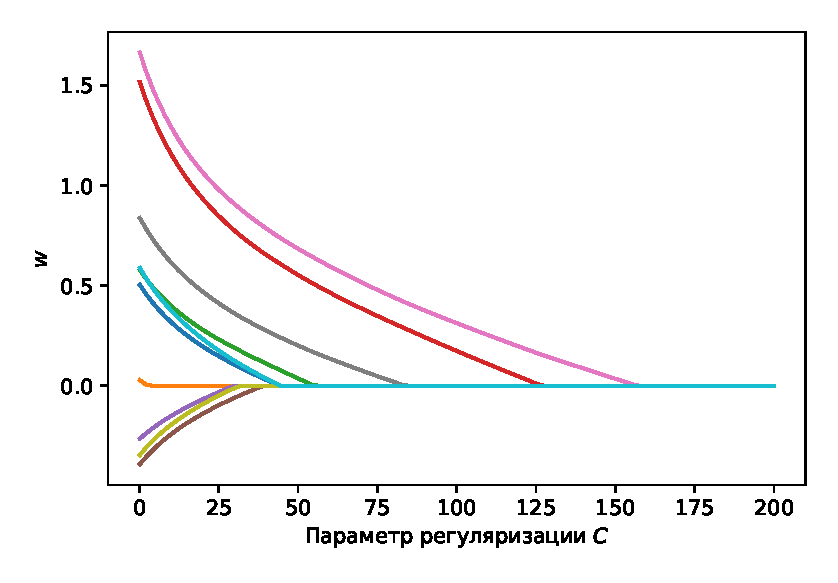
\includegraphics[width=0.5\textwidth]{../figures/log_reg_cs_exp.eps}
	\caption{Sample figure caption.}
	\label{fig:fig1}
\end{figure}

\subsection{Tables}
See awesome Table~\ref{tab:table}.

The documentation for \verb+booktabs+ (`Publication quality tables in LaTeX') is available from:
\begin{center}
	\url{https://www.ctan.org/pkg/booktabs}
\end{center}


\begin{table}
	\caption{Sample table title}
	\centering
	\begin{tabular}{lll}
		\toprule
		\multicolumn{2}{c}{Part}                   \\
		\cmidrule(r){1-2}
		Name     & Description     & Size ($\mu$m) \\
		\midrule
		Dendrite & Input terminal  & $\sim$100     \\
		Axon     & Output terminal & $\sim$10      \\
		Soma     & Cell body       & up to $10^6$  \\
		\bottomrule
	\end{tabular}
	\label{tab:table}
\end{table}

\subsection{Lists}
\begin{itemize}
	\item Lorem ipsum dolor sit amet
	\item consectetur adipiscing elit.
	\item Aliquam dignissim blandit est, in dictum tortor gravida eget. In ac rutrum magna.
\end{itemize}


\bibliographystyle{unsrtnat}
\bibliography{references}

\end{document}